\part{Diskontinuierliche Gruppen}


% ==========
\section{Möbiustransformationen}\label{sec_moebius}

\DB Es sei $X$ ein topologischer Raum und $G$ eine Gruppe von
Homöomorphismen von $X$, die effektiv operiert.
\begin{enumerate}
\item $G$ \emph{operiert diskontinuierlich}\index{diskontinuierlich}\index{Aktion!diskontinuierlich}
in $x\in X$, wenn es
eine offene Umgebung $U$ von $x$ gibt mit $g(U)\cap U=\emptyset$
für alle bis auf endlich viele $g\in G$.
\item $G$ heißt \emph{diskontinuierlich}\index{diskontinuierlich}\index{Gruppe!diskontinuierlich},
wenn es ein $x\in X$ gibt, so dass $G$ in $x$ diskontinuierlich
operiert.
\item Die Menge der \emph{gewöhnlichen Punkte}\index{gewöhnliche Punkte},
\[
\Omega(G) := \{x\in X : G \text{ operiert diskontinuierlich in } x \},
\]
ist eine offene, $G$-invariante Teilmenge von $X$.
Es ist $U\subseteq \Omega(G)$.\index{$\Omega(G)$ (gewöhnliche Punkte)}
\end{enumerate}

\BSP Diskontinuierliche Gruppen.
\begin{enumerate}
\item Es sei $X=\hat{\CC}:=\PP^1(\CC)$ die
\emph{Riemannsche Zahlenkugel}.\index{Riemannsche Zahlenkugel}\index{$\hat{\CC}$ (Riemmansche Zahlenkugel)}
Es sei $g\in\PGL_2(\CC)$ und $G=\lag g\rag$.
\begin{enumerate}
\item $g$ ist hyperbolisch.
Dann ist $g$ konjugiert zu $z\mapsto \lambda z$ mit $\lambda\in\CC$,
$|\lambda|>1$.
Setze $U:=\{z\in\CC : 1<|z|<|\lambda| \}$.
In der folgenden Skizze ist $\lambda=\frac{5}{3}$.
\begin{center}
	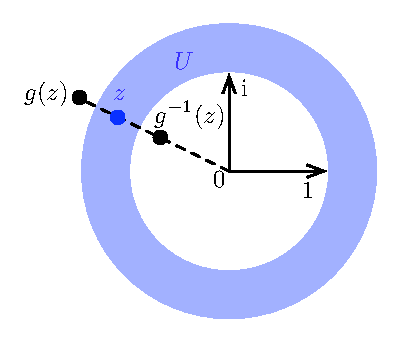
\includegraphics{grugraImages/UinC}
\end{center}
Für $z\in U$ und $n\in\ZZ$ ist $g^n(z)=\lambda^n z$,
also
\[
|g^n(z)|=|\lambda|^n |z|=
\left\{
\begin{matrix}
>|\lambda|, & n\geq 1 \\
< 1, & n\leq -1 \\
|z|, & n=0
\end{matrix}
\right..
\]
Also ist $g^n(U)\cap U=\emptyset$ für $n\neq 0$.
Damit ist $G$ diskontinuierlich und es ist
$\Omega(G)=\hat{\CC}\backslash\{0,\infty\}$.
Der Bahnenraum $\Omega(G)/G$ ist ein Torus, den man durch
Identifizieren des inneren und des äußeren Randes von $U$
erhält.
\begin{center}
	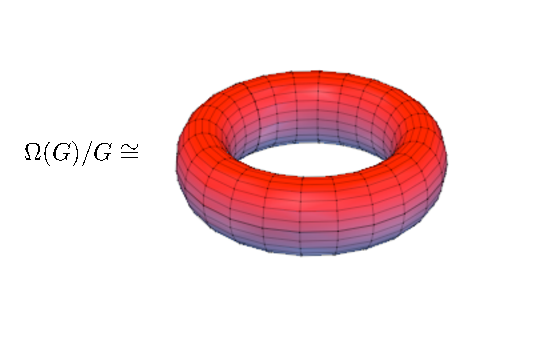
\includegraphics{grugraImages/Torus.pdf}
\end{center}
Die Projektion $\Omega(G)\Ra\Omega(G)/G$ ist ein
lokaler Homöomorphismus.
\item $g$ ist elliptisch.
Dann ist $g$ konjugiert zu $z\mapsto\lambda z$ mit $|\lambda|=1$.\\
Ist $\lambda$ eine $n$-te Einheitswurzel, so ist $G$ endlich und
operiert somit diskontinuierlich auf $\hat{\CC}$.
Es ist $\hat{\CC}/G\cong\hat{\CC}$.\\
Ist $\lambda$ keine Einheitswurzel, so ist $G$ unendlich und
$G\cong\ZZ$. Jeder Punkt des Einheitskreises $\{z\in\CC:|z|=1\}$
ist ein Häufungspunkt von $\{\lambda^n:n\in\ZZ\}$, denn ist
$\lambda_0$ ein Häufungspunkt, so gibt es eine Folge
$(\lambda^{n_i})_i$ mit $\lambda^{n_i}\Ra\lambda_0$,
und damit gilt auch $\lambda^{-n_{i+1}}\lambda^{n_i}\Ra 1$.
Es folgt nun, dass $G$ in keinem Punkt diskontinuierlich operiert,
da für $z\in\hat{\CC}$ die Folge $g^{-n_{i+1}}g^{n_i}(z)$ gegen
$z$ konvergiert.
\item $g$ ist parabolisch.
Dann ist $g$ konjugiert zu $z\mapsto z+1$, und $G\cong \ZZ$ ist
diskontinuierlich auf
$U:=\{z\in\CC:-\frac{1}{2}<\Re(z)<\frac{1}{2}\}$.
Es ist $\Omega(G)=\hat{\CC}\backslash\{\infty\}$.
Man erhält den Bahnenraum $\Omega(G)/G$, indem man die Ränder
des Streifens $U$ miteinander identifiziert und in dem so 
erhaltenen Zylinder die \glqq Ränder im Unendlichen\grqq\
miteinander identifiziert, also zu einem Punkt zusammenzieht.
\begin{center}
	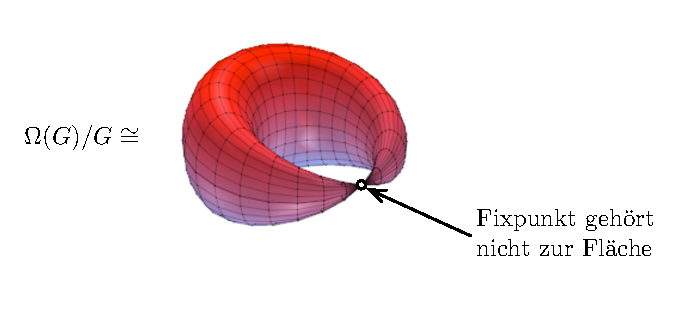
\includegraphics{grugraImages/cuspTorus}
\end{center}
Dieser Punkt entspricht für $z\mapsto z+1$ dem Fixpunkt $\infty$
und gehört nicht zur Fläche $\Omega(G)/G$.
Wählt man ein zu $z\mapsto z+1$ konjugiertes $g$ derart, dass
$0$ der Fixpunkt ist, so erhält man als Projektion
\[
\CC\cong \Omega(G) \Ra \Omega(G)/G\cong \CC^\times,\quad
z\mapsto \e^{2\pi\i z}.
\]
\end{enumerate}
\item Ähnlich wie für $\hat{\CC}$ können wir die Aktion von
$g\in\PGL_2(\QQ_p)$ auf $\PP^1(\QQ_p)$ betrachten.
Es sei $G=\lag g\rag$.
\begin{enumerate}
\item $g$ ist hyperbolisch. Wie im komplexen Fall ist $g$ konjugiert
zu $z\mapsto\lambda z$ mit $|\lambda|>1$, und $G$ ist diskret.
Es ist $\Omega(G)=\PP^1(\QQ_p)\backslash\{\text{Fixpunkte von }g\}$.
\item $g$ ist elliptisch. $G$ ist genau dann diskret, wenn
$g$ von endlicher Ordnung ist.
\item $g$ ist parabolisch. Dann ist $g$ konjugiert zu $z\mapsto z+1$.
Für jedes $z\in\QQ_p$ konvergiert $g^{p^n}(z)=z+p^n$ gegen $z$.
In jeder Umgebung von $z$ gibt es also unendlich viele $g^{p^n}$
und somit ist $G$ nicht diskontinuierlich.
\end{enumerate}
\end{enumerate}

\SATZ Es sei $\KK$ ein Körper der Charakteristik $0$ und
$G<\PGL_2(\KK)$ eine endliche Untergruppe.
Dann ist $G$ isomorph zu einer der folgenden Gruppen:
\begin{enumerate}
\item $\ZZ/n\ZZ$ mit $n\geq 1$.
\item $\mathrm{D}_n$ (Diedergruppe) mit $n\geq 1$.\index{Diedergruppe}
\item $\mathrm{A}_4$ (Tetraedergruppe).\index{Tetraedergruppe}
\item $\sym_4$ (Oktaedergruppe).\index{Oktaedergruppe}
\item $\mathrm{A}_5$ (Ikosaedergruppe).\index{Ikosaedergruppe}
\end{enumerate}
\bew Ohne Einschränkung nehmen wir an, dass jedes $g\in G$ zwei
Fixpunkte in $\PP^1(\KK)$ hat (notfalls müssten wir zu einer
endlichen Körpererweiterung von $\KK$ übergehen, um dies zu
gewährleisten). Es sei $n=|G|$ und $Z=\{z_1,\ldots,z_m\}$
die Menge der Fixpunkte von Elementen aus $G\backslash\{\id\}$.
Dann operiert $G$ auf $Z$: Ist $z_i$ Fixpunkt von $h$, und ist
$g\in G$, so ist $g(z_i)$ ein Fixpunkt von $ghg^{-1}$.\\
Es seien nun $z_1,\ldots,z_s$ Vertreter der $G$-Bahnen.
Setze $\nu_i=|G_{z_i}|$, d.h. es ist $|G z_i|=\frac{n}{\nu_i}$
(beachte: $\nu_i|n$). Es gilt
\[
2n-2 = \SUM{s}{i=1}(\nu_i-1)\frac{n}{\nu_i},
\]
was äquivalent ist zu
\[
1\leq 2-\frac{2}{n} = \SUM{s}{i=1}\left(1-\frac{1}{\nu_i}\right)
\leq 2.
\]
Gesucht ist eine Lösung dieser Gleichung, die die Bedingungen
$n,\nu_i\in\NN$, $\nu_i\geq 2$, $\nu_i|n$ erfüllt.
Die Fälle $s=1$ und $s\geq 4$ lassen sich direkt ausschließen,
da hier die rechte Seite der Gleichung $<1$ bzw. $>2$ ist.
\begin{enumerate}
\item[]$s=2$: Es ist
$2-\frac{2}{n}=2-\frac{1}{\nu_1}-\frac{1}{\nu_2}$, und da $\nu_i|n$
gilt, folgt $\nu_1=\nu_2=n$. Somit haben alle Elemente die selben
Fixpunkte, es ist $G\cong\ZZ/n\ZZ$.
\item[]$s=3$: Ohne Einschränkung sei $\nu_1\leq\nu_2\leq\nu_3$.
Dann ist
\[
3-\frac{1}{\nu_1}-\frac{1}{\nu_2}-\frac{1}{\nu_3}=2-\frac{2}{n}
\ \lra\ 
\frac{1}{\nu_1}+\frac{1}{\nu_2}+\frac{1}{\nu_3}=1+\frac{2}{n}.
\]
Damit muss $\nu_1=2$ sein, sonst wäre die linke Seite der Gleichung
zu klein. Ebenso muss $\nu_2\leq 3$ sein.
\begin{itemize}
\item[]$\nu_2=2$: Es ist $\nu_3=\frac{n}{2}$, d.h. $G$ enthält
ein Element $\tau$ von Ordnung $\frac{n}{2}$ und ein Element
$\sigma$ von Ordnung $2$ mit $\sigma\tau\sigma=\tau^{-1}$
($\sigma$ vertauscht die Fixpunkte von $\tau$).
Es ist also $\lag\sigma,\tau\rag\cong\mathrm{D}_{\frac{n}{2}}$.
\item[] $\nu_2=3$: Es muss $\nu_3\in\{3,4,5\}$ sein.
Für $\nu_3=3$ ist $G\cong\mathrm{A}_4$ und $n=12$.
Für $\nu_3=4$ ist $G\cong\sym_4$ und $n=24$.
Für $\nu_3=5$ ist $G\cong\mathrm{A}_5$ und $n=60$.
\qed
\end{itemize}
\end{enumerate}


% ==========
\section{Diskontinuierliche Untergruppen von $\PGL_2(\QQ_p)$}\label{sec_disUG}

\BEM Es sei $\KK$ ein bewerter Körper, etwa $\KK=\CC$ oder $\KK=\QQ_p$ 
(vgl. van der Waerden \cite{vdW}, § 141).
Dann gilt:
\begin{enumerate}
\item $\PP^1(\KK)$ ist ein Hausdorff-Raum.
\item $\PGL_2(\KK)$ ist eine topologische Gruppe, d.h. die
Abbildungen $(g_1,g_2)\mapsto g_1 g_2$ und $g\mapsto g^{-1}$
sind stetig.\index{topologische Gruppe}\index{Gruppe!topologisch}
\end{enumerate}
\bew \begin{enumerate}
\item Eine Umgebungsbasis für $\infty$ ist durch die Mengen
$U_r=\{z\in\KK:|z|>r\}$ mit $r>0$ gegeben.
\item Wir können $\GL_2(\KK)$ als die offene Teilmenge
$\{(a,b,c,d)\in\KK^4 : ad-bc \neq 0 \}$ von $\KK^4$ auffassen.
Dann bekommt $\PGL_2(\KK)$ die Quotiententopologie, d.h.
\[
d(g_1,g_2) < \eps \quad \lra \quad
\exists A_1\in g_1, A_2\in g_2 :
\|A_1-A_2\| < \eps
\]
für eine beliebige Norm von $\KK^4$.
Dies ist verträglich mit Multiplikation und Inversion.
\qed
\end{enumerate}

\BEM\label{bem_diskret}
Ist $G<\PGL_2(\KK)$ diskontinuierlich, so ist $G$ diskret 
als Teilmenge von $\PGL_2(\KK)$ (d.h. $G$ hat keinen Häufungspunkt
in $\PGL_2(\KK)$).

\bew Zunächst stellen wir fest, dass $G<\PGL_2(\KK)$ genau dann
diskret ist, wenn $\id$ kein Häufungspunkt von $G$ ist. Wäre nämlich
$g\in\PGL_2(\KK)$ ein Häufungspunkt von $G$, d.h. gäbe es eine
Folge $(g_i)$ mit $g_i\Ra g$ und $g_i\neq g_j$ für $i\neq j$, so
konvergierte $g_{i+1}^{-1} g_i$ nach $g^{-1}g=\id$, da die
Gruppenverknüpfungen stetig sind.

Es reicht also im Folgenden zu zeigen, dass $\id$ kein Häufungspunkt
ist. Dazu sei $G$ nun eine nicht-diskrete Untergruppe.
Es gibt also eine Folge $(g_i)$, die gegen $\id$ konvergiert.
Dann ist auch $g_i(x)=x$ für jedes $x\in\PP^1(\KK)$, und für jede
Umgebung $U$ von $x$ ist $g_i(U)\cap U\neq\emptyset$ für unendlich
viele $i$. Also operiert $G$ nicht diskontinuierlich in allen
$x\in\PP^1(\KK)$.
\qed

\BEM\label{bem_lokalkompakt}
Es sei $\KK$ ein bewerteter und lokalkompakter Körper, $G$ eine
diskontinuierliche Untergruppe von $\PGL_2(\KK)$
und $\infty\in\Omega(G)$.
Dann ist für jede Konstante $C>0$ die Menge
\[
\Bigl\{ c\in\KK: \text{ es gibt }
\begin{pmatrix}
a & b \\ c & d
\end{pmatrix}\in G
\text{ mit }
|c|<C
\Bigr\}
\]
endlich.

\bew Wir nehmen an,
$g_n=\begin{pmatrix}
a_n & b_n \\ c_n & d_n
\end{pmatrix}$ sei eine Folge in $G$ mit $|c_n|<C$ und $g_n\neq g_m$
für $n\neq m$. Da $\KK$ lokalkompakt ist, hat $(c_n)$ einen 
Häufungspunkt, also gelte ohne Einschränkung $c_n\Ra c$ (ansonsten
wähle eine konvergente Teilfolge von $(c_n)$).
Wegen $\infty\in\Omega(G)$ ist die Folge $\frac{a_n}{c_n}=g_n(\infty)$
beschränkt, also ohne Einschränkung $a_n\Ra a$.
Ebenso ist $-\frac{d_n}{c_n}=g_n^{-1}(\infty)$ beschränkt,
also ohne Einschränkung $d_n\Ra d$. Auch $\frac{b_n}{d_n}=g_n(0)$
ist beschränkt, da sonst in jeder Umgebung von $\infty$
unendlich viele $G$-äquivalente Punkte liegen, also
ohne Einschränkung $b_n\Ra b$.
Es folgt $a_n d_n - b_n c_n \Ra ad-bc=1$ und
$\begin{pmatrix}
a_n & b_n \\ c_n & d_n
\end{pmatrix}\Ra
\begin{pmatrix}
a & b \\ c & d
\end{pmatrix}\in\SL_2(\KK)$.
Dies ist nach Bemerkung \ref{bem_diskret} ein Widerspruch zur
Diskontinuität von $G$.
\qed

\FOLG\label{folg_diskont}
Ist $G<\PGL_2(\QQ_p)$ diskontinuierlich, so ist für jede
Ecke $x\in E(T_p)$ die Fixgruppe $G_x$ endlich.

\bew Ohne Einschränkung können wir Folgendes annehmen:
\begin{itemize}
\item $G<\PSL_2(\QQ_p)$ (sonst ersetze $\QQ_p$ durch den Körper $\KK$
mit $[\KK:\QQ_p]=4$, in dem alle quadratischen Polynome über $\QQ_p$
zerfallen).
\item
$x=\KU_1(0)$ (sonst wähle $g\in\PGL_2(\QQ_p)$ mit $g(x)=\KU_1(0)$
und betrachte $g G_x g^{-1}=(gGg^{-1})_{\KU_1(0)}$).
\item $\infty\in\Omega(G)$ (sonst finde für $z\in\Omega(G)$ ein
$g\in\PGL_2(\ZZ_p)$ mit $g(z)=\infty$ und ersetze $G$ durch
$gGg^{-1}$).
\end{itemize}
Nach Bemerkung \ref{bem_lokalkompakt} enthält $G$ nur endlich viele
Elemente $\begin{pmatrix}
a & b \\ c & d
\end{pmatrix}$ mit $|c|\leq 1$, also auch $c\in\ZZ_p$.
Der Stabilisator von $\KU_1(0)$ ist nach Proposition \ref{prop_stab_K}
aber gerade $\PSL_2(\ZZ_p)$.
\qed

\BEM\label{bem_TpG}
Ist $G$ eine endlich erzeugte Untergruppe von $\PGL_2(\QQ_p)$,
so gibt es in $T_p$ einen $G$-invarianten Teilbaum $T_p(G)$, so dass
$T_p(G)/G$ ein endlicher zusammenhängender Graph ist.

\bew Es seien $g_1,\ldots, g_n$ die Erzeuger von $G$ und so geordnet,
dass $g_1,\ldots,g_k$ hyperbolisch und $g_{k+1},\ldots,g_n$
elliptisch oder parabolisch sind.
Ohne Einschränkung habe jedes $g_j$, $j=k+1,\ldots,n$, einen Fixpunkt
$x_j$ in $T_p$.
Für jedes hyperbolische $g_i$ sei $F_i$ ein Abschnitt in der Achse
$A_{g_i}$ mit Anfangspunkt $x_i$ und Endpunkt $g_i(x_i)$.
Es sei $F$ der von den $F_i$ und den $x_j$ aufgespannte Teilbaum
von $T_p$, und
\[
T_p(G)/G := \BCUP{}{g\in G} g(F).
\]
Dieser Graph ist nach Konstruktion $G$-invariant.
$T_p(G)$ ist zusammenhängend, da für jedes $i=1,\ldots,n$ gilt:
\[
F \cap g_i(F) \neq \emptyset,
\]
und mit Induktion über die Länge $\ell(g)$ von $g\in G$ als Wort in
$g_1,\ldots,g_n$ folgt, dass $T_p(G)$ zusammenhängend ist.
\qed

Wir kombinieren die Endlichkeitsaussagen der Bemerkungen
\ref{bem_lokalkompakt} und \ref{bem_TpG} im folgenden Satz.

\SATZ Es sei $G$ eine endlich erzeugte diskontinuierliche
Untergruppe von $\PGL_2(\QQ_p)$. Dann gilt:
\begin{enumerate}
\item $G$ ist isomorph zur Fundamentalgruppe eines endlichen Graphen
von endlichen Gruppen.
\item $G$ ist \emph{virtuell frei}\index{virtuell frei}\index{Gruppe!virtuell frei},
d.h. $G$ enthält eine
freie Untergruppe, die ein Normalteiler von endlichem Index ist.
\end{enumerate}
\bew
\begin{enumerate}
\item Dies folgt aus Bemerkung \ref{bem_TpG}, Folgerung
\ref{folg_diskont} und Satz \ref{satz_cover}.
\item Folgt aus Teil 1 und dem folgenden Satz
\ref{satz_virtuell_frei}.
\qed
\end{enumerate}

\SATZ \label{satz_virtuell_frei}
Ist $G$ die Fundamentalgruppe eines endlichen, zusammenhängenden
Graphen $\GG=(\GR,G_x,G_k,\alpha_k)$ von endlichen Gruppen, so ist $G$
virtuell frei.

\bew Induktion über die Anzahl $n$ der Kanten von $\GR$.

$n=0$: In diesem Fall ist nichts zu zeigen.

$n\geq 1$: Es sei $k\in K(\GR)$ und $\GR'=\GR-k$.
Wir unterscheiden nun die Fälle, dass $\GR'$ zusammenhängend ist
oder nicht.
\begin{enumerate}
\item $\GR'$ ist zusammenhängend. Es sei $G'$ die
Fundamentalgruppe des Graphen von Gruppen zu $\GR'$ und $C=G_k$.
Dann ist $G=\HNN(G',C,\alpha_k,\alpha_{\bar{k}})$.
\item $\GR'$ ist nicht zusammhängend. Dann ist die $\GR'$
die disjunkte Vereinigung $\GR'=\GR'_1 \os{\cup}{.} \GR'_2$.
In diesem Fall seien $G_1$ und $G_2$ die Fundamentalgruppen von
$\GR'_1$ bzw. $\GR'_2$ und $C=G_k$.
Es ist $G=G_1 *_C G_2$.
\end{enumerate}
Nach Induktionsvoraussetzung haben $G'$ bzw. $G_1$ und $G_2$ freie
Normalteiler $F'$ bzw. $F_1$ und $F_2$ von endlichem Index.
Je nach Fall sei nun $A=G'/F'$ bzw. $A=G_1/F_1$ und $B=G_2/F_2$.
Weiter seien $p_A$ bzw. $p_B$ die entsprechenden 
Restklassenhomomorphismen. Dann sind $p_A|_{\alpha_k(C)}$ und
$p_B|_{\alpha_{\bar{k}}(C)}$ injektiv (da die endliche Gruppe
$\alpha_k(C)$ nur trivialen Schnitt mit dem freien Kern der
Abbildung haben kann).\\
Im ersten Fall induziert $p_A$ einen Homomorphismus
\[
p:G\Ra\HNN(A,C,p_A\circ\alpha_k,p_A\circ\alpha_{\bar{k}})
=
\lag G',t | t\alpha_k(c) t^{-1}=\alpha_{\bar{k}}(c)\
\forall c\in C\rag.
\]
Im zweiten Fall induzieren $p_A$ und $p_B$ einen Homomorphismus
\[
p:G\Ra A *_C B.
\]
Ist $H\leq G$ eine endliche Untergruppe, so ist $H\cap\K{p}=\{1\}$,
denn $H$ ist konjugiert zu einer Untergruppe von $G'$ bzw. von 
$G_1$ oder $G_2$, aber $\K{p}\cap G_1=\K{p}\cap F_1$.
Wir verwenden die folgenden Behauptungen, die im Anschluss an den
Beweis des Satzes bewiesen werden:
\begin{enumerate}
\item Im ersten Fall gibt es eine endliche Gruppe $G_0$ und einen
Homomorphismus
$\phi:\HNN(A,C,p_A\circ\alpha_k,p_B\circ\alpha_{\bar{k}})\Ra G_0$,
so dass $\phi|_A$ injektiv ist.
\item Im zweiten Fall gibt es eine endliche Gruppe $G_0$ und einen
Homomorphismus $\phi:A*_C B\Ra G_0$, so dass $\phi|_A$ und $\phi|_B$
injektiv sind.
\end{enumerate}
Dann setzen wir $\rho:=\phi\circ p:G\Ra G_0$. Es gilt, dass $\rho|_H$
injektiv ist für alle endlichen Untergruppen $H\leq G$.
Also ist $\K{\rho}$ ist ein Normalteiler von endlichem Index,
da das Bild endlich ist. Im zweiten Fall folgt aus
Folgerung \ref{folg_H_frei}, dass $\K{\rho}$ frei ist.
Im ersten Fall kann man dies aus einer analogen Aussagen für
die HNN-Erweiterung folgern.

Damit ist der Satz bewiesen und es bleibt die Existenz von $G_0$
und $\phi$ zu zeigen. Wir beginnen mit dem zweiten Fall:\\
Dazu seien $A/C=\{\bar{a}_1,\ldots,\bar{a}_d\}$ und
$B/C=\{\bar{b}_1,\ldots,\bar{b}_e\}$ die Mengen der Rechtsnebenklassen
(eigentlich: $A/(p_A\circ\alpha_k(C))$ und
$B/(p_B\circ\alpha_{\bar{k}}(C))$), und $X$ sei die Menge
\[
X = A/C \times C \times B/C.
\]
Dann ist
\[
A/C \times C \Ra A, \quad (\bar{a}_i,c)\mapsto a_i c
\]
eine bijektive Abbildung. $A$ operiert auf $A/C\times C$ durch
Rechtsmultiplikation,
d.h. $a\cdot(\bar{a}_i,c)=(\bar{a}_j,\tilde{c})$, wenn
$a_j\tilde{c}=a_i c a$ gilt, insbesondere ist
$c'\cdot(\bar{a}_i,c)=(\bar{a}_i,cc')$ für $c'\in C$.
Somit operiert $A$ auch auf $X$ durch
$a\cdot(\bar{a}_i,c,\bar{b}_j)=(a\cdot(a_i,c),\bar{b}_j)$.
Entsprechend operiert $B$ auf $C\times B/C$ durch
$b\cdot(c,\bar{b}_j)=(\tilde{c},\bar{b}_k)$, wenn
$b_k\tilde{c}=b_j c b$. Ebenso operiert $B$ auf $X$.
Wir erhalten so injektive Homomorphismen
$\psi_A:A\Ra\mathrm{Perm}(X)$ und $\psi_B:B\Ra\mathrm{Perm}(X)$ mit
$\psi_A\circ\alpha_k=\psi_B\circ\alpha_{\bar{k}}$.
Wähle also $G_0=\mathrm{Perm}(X)$. Durch die UAE von $A*_C B$
erhalten wir einen eindeutigen Homomorphismus $\phi$ mit
$\phi|_A=\psi_A$ und $\phi|_B=\psi_B$.

Nun zeigen wir die Existenz von $G_0$ und $\phi$ für den ersten
Fall:\\
Dazu seien $C_1=\alpha_k(C)$, $C_2=\alpha_{\bar{k}}(C)$ und
$\psi:=\alpha_{\bar{k}}\circ\alpha_k^{-1}:C_1\os{\Ra}{\sim} C_2$.
Weiter seien $a_1,\ldots,a_d$ Repräsentanten von $A/C_1$ und
$a'_1,\ldots,a'_d$ Repräsentanten von $A/C_2$. Jedes $a\in A$ hat
also eine eindeutige Darstellung $a=a_i c$ für ein $i$ und $c\in C_1$.
Somit ist die Abbildung
\[
\theta:A\Ra A,\quad a=a_i c \mapsto a_i' \psi(c)
\]
bijektiv.
Für $a\in A$ und $c'\in C_1$ ist
\begin{align*}
\theta(ac') &= \theta(a_i c c') \\
&= a'_i \psi(cc') \\
&= a'_i \psi(c)\psi(c') \\
&= \theta(a)\psi(c'). \qquad (*)
\end{align*}
Wähle nun $G_0=\mathrm{Perm}(A)$ und definiere
$\phi:\HNN(A,C,\alpha_k,\alpha_{\bar{k}})\Ra G_0$ durch
\begin{align*}
\phi(a)(a')&=a' a\quad \text{ für alle } a,a'\in A, \\
\phi(t)&=\theta.
\end{align*}
$\phi$ ist wohldefiniert: Für $c\in C_1$ ist $tct^{-1}=\psi(c)$.
Für $a\in A$ ist
\begin{align*}
\phi(tct^{-1})(a) &= \theta(\phi(c)(\theta^{-1}(a))) \\
&= \theta(\theta^{-1}(a)c) \\
&\us{=}{(*)} \theta(\theta^{-1}(a)) \psi(c) \\
&= a \psi(c).
\end{align*}
Damit ist alles gezeigt.
\qed

\BSP Als Beispiel zur Konstruktion von $G_0$ und $\phi$ aus
dem Beweis von Satz \ref{satz_virtuell_frei} betrachten wir
\[
\ZZ/4\ZZ *_{\ZZ/2\ZZ} \ZZ/6\ZZ \cong \SL_2(\ZZ).
\]
Schreiben wir $\ZZ/4\ZZ=\{1,a,c,ac\}$ und
$\ZZ/6\ZZ=\{1,b,b^2,c,bc,b^2c\}$, so ist
\[
X = \{1,a\} \times \{1,c\} \times \{1,b,b^2\}.
\]
Es ist $|X|=12$, also $G_0=\sym_{12}$. Es ist $\B{\phi}=\ZZ/12\ZZ$.

Ohne Beweis stellen wir fest, dass auch die Umkehrung
von Satz \ref{satz_virtuell_frei} gilt.
\SATZ Eine endlich erzeugte Gruppe ist genau dann virtuell frei,
wenn sie Fundamentalgruppe eines zusammenhängenden, endlichen
Graphen von endlichen Gruppen ist.
